\chapter{Results and Discussion }

\section{Introduction}
 This section presents a comprehensive analysis of selected articles examining how work-related stress, dietary habits, and physical activity levels influence metabolic syndrome development and progression among working adults. The analysis is based on systematic review methodology and encompasses publication trends, demographic characteristics, measurement approaches, and study design patterns.
 
 \section{Results}
 \subsection{Description of Included Studies}
 In this study, an extensive search was carried out in three databases, resulting in a total of 1214 articles. Following the removal of ineligible and duplicate articles, 767 unique articles were retained. These articles were first assessed on the basis of their titles and abstracts, leading to the identification of 184 relevant studies. 94 articles could be retrieved. After thorough examination of the remaining 90 articles, only 27 articles qualified for included studies. A visual representation of this selection is presented in Figure~ \ref{fig:prisma-flow-diagram2}.
\begin{figure}[H]
    \centering
    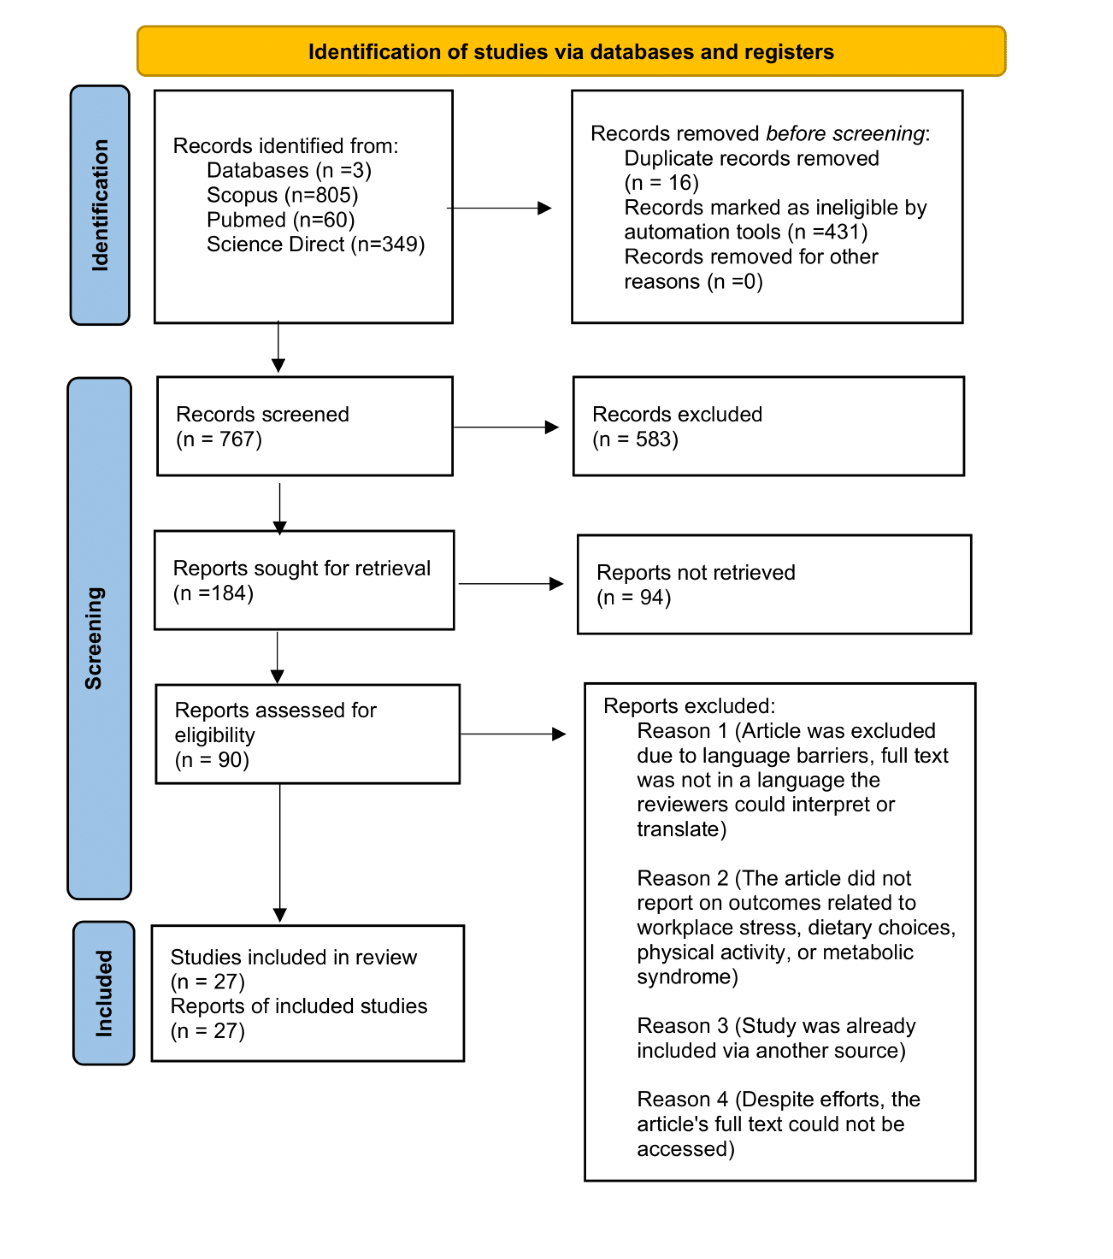
\includegraphics[width=\linewidth]{PRISMA_2020_flow_diagram_new_SRs_v1-1 (1).png}
    \caption{PRISMA  flow diagram for findings.}
    \label{fig:prisma-flow-diagram2}
\end{figure}

 \subsection{Publication Trends and Research Evolution}
 The analysis of publication patterns from 2015 to 2024 reveals significant fluctuations in research activity regarding metabolic syndrome and its workplace-related determinants (Figure ~\ref{fig:prisma-flow-diagram}). The field demonstrates three distinct peaks in research output: 2017 (4 publications), 2020 (5 publications), and 2024 (4 publications), with 2020 representing the highest research activity.
 \begin{figure}[H]
    \centering
    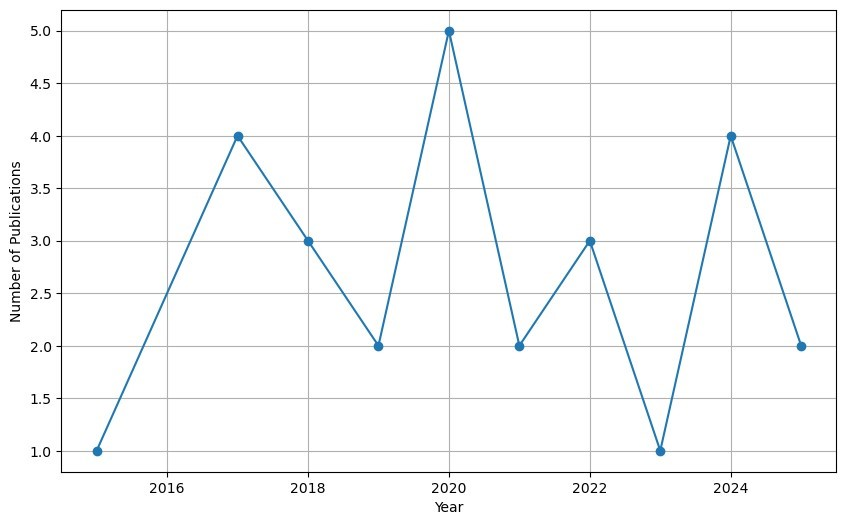
\includegraphics[width=\linewidth]{Number of Publications by Year.jpg}
    \caption{Number of Publications by Year}
    \label{fig:prisma-flow-diagram}
\end{figure}
 The notable peak in 2020 coincides with heightened awareness of workplace health issues during the COVID-19 pandemic, suggesting increased recognition of the interconnected relationships between occupational stress, lifestyle factors, and metabolic health. The sustained interest through 2024 indicates continued relevance of this research domain. The cyclical pattern observed, with periods of intensive research followed by relative decreases, reflects the evolving nature of workplace health research and may correspond to funding cycles or emerging health priorities.

\subsection{Geographic Distribution and International Research Patterns}
The geographic analysis reveals a concentrated research landscape with notable international collaboration patterns (Figure ~\ref{fig:prisma-flow-diagram3}). The United States leads in research output with 5 studies, followed by Italy with 4 studies. This distribution suggests a strong research infrastructure and funding support in these regions for research on metabolic syndrome in the workplace.
\begin{figure}[H]
    \centering
    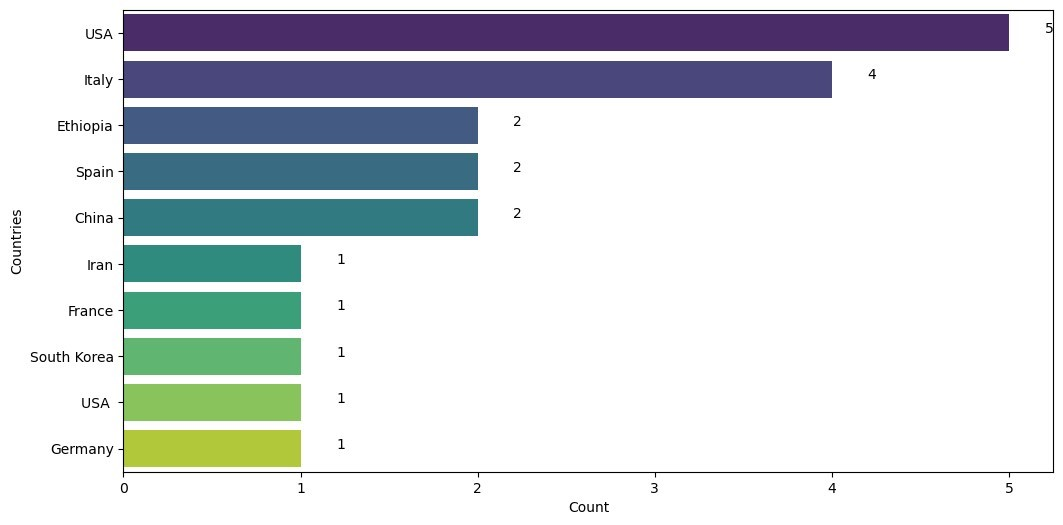
\includegraphics[width=\linewidth]{Geographic.jpg}
    \caption{Geographic Distribution of Research Studies}
    \label{fig:prisma-flow-diagram3}
\end{figure}
 Ethiopia, Spain, and China each contribute 2 studies, indicating emerging research capacity in diverse global contexts. Single-study contributions from Iran, France, South Korea, and Germany demonstrate widespread international interest in workplace metabolic health research. The geographic diversity suggests that metabolic syndrome in workplace settings is recognized as a global health challenge requiring culturally adapted interventions and context-specific research approaches.

 \subsection{Workplace Settings and Research Environments}
 The analysis of the research settings in Figure~\ref{fig:prisma-flow-diagram4} reveals a strong concentration in academic settings, with 11 studies conducted in academic settings. This predominance reflects the accessibility of academic populations for research participation and the established research infrastructure within universities and educational institutions.
 \begin{figure}[H]
    \centering
    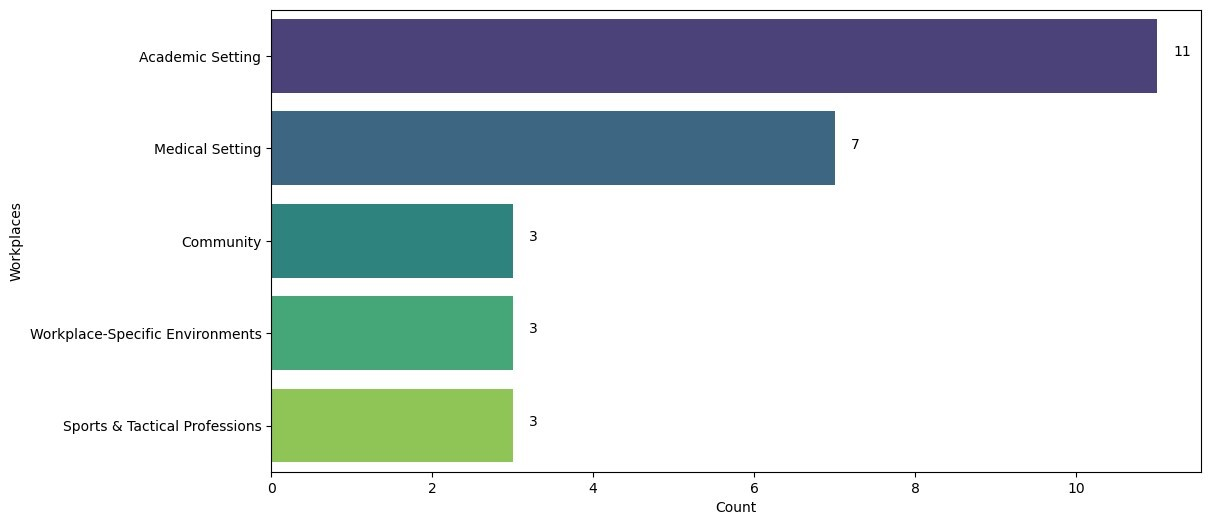
\includegraphics[width=\linewidth]{workplace.jpg}
    \caption{Distribution of Workplace Research settings}
    \label{fig:prisma-flow-diagram4}
\end{figure}
Medical settings comprise the second-largest category with 7 studies, indicating recognition of metabolic syndrome risks among healthcare workers. The high-stress nature of medical environments and irregular work schedules make healthcare settings particularly relevant for studying workplace-related metabolic dysfunction.\\
Community settings, workplace-specific environments, and sports and tactical professions each contribute 3 studies. The inclusion of sports and tactical professions is particularly noteworthy, as these populations face unique occupational stressors and physical demands that may influence metabolic health outcomes differently than traditional office environments. The limited representation of diverse workplace settings suggests a need for broader occupational health research across various industries and job categories.

\subsection{Workplace Stress Assessment Patterns}
The analysis of stress assessment approaches reveals significant methodological limitations in current research (Figure ~\ref{fig:prisma-flow-diagram5}). In particular, 11 studies did not assess stress at all, representing a critical gap given the central role of workplace stress in the development of metabolic syndromes. This omission limits understanding of stress-mediated pathways to metabolic dysfunction.
\begin{figure}[H]
    \centering
    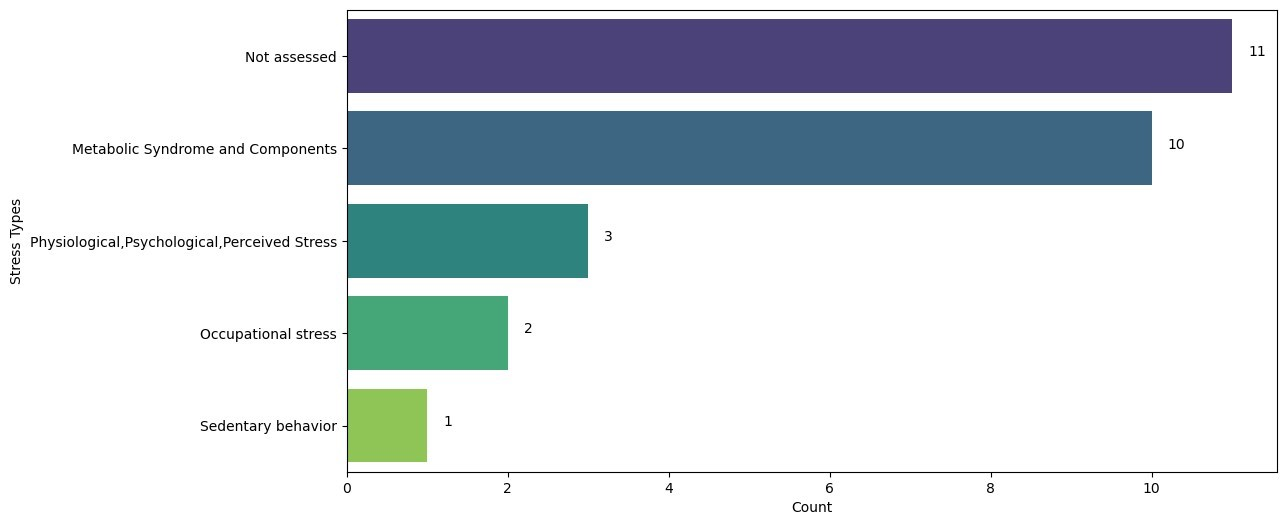
\includegraphics[width=\linewidth]{type of stress.jpg}
    \caption{Types of Stress Assessment In Research Studies}
    \label{fig:prisma-flow-diagram5}
\end{figure}
Among the studies that assessed stress, components of metabolic syndrome were measured in 10 studies, although this represents outcome measurement rather than stress assessment. Only 3 studies comprehensively examined physiological, psychological, and perceived stress, while 2 studies specifically focused on occupational stress. One study addressed sedentary behavior as a stress-related factor.\par
The predominance of studies without stress assessment represents a significant methodological limitation, particularly given the established pathways linking chronic workplace stress to insulin resistance, cortisol dysregulation, and metabolic dysfunction. This pattern suggests that current research may underestimate the role of stress-mediated mechanisms in workplace-related metabolic syndrome.

\subsection{Gender Distribution and Research Inclusion}
The gender distribution analysis in Figure ~\ref{fig:prisma-flow-diagram6} reveals that the majority of the studies (21) included both male and female participants, demonstrating good research inclusion and recognition of potential gender differences in the development of metabolic syndromes and workplace stress responses.
\begin{figure}[H]
    \centering
    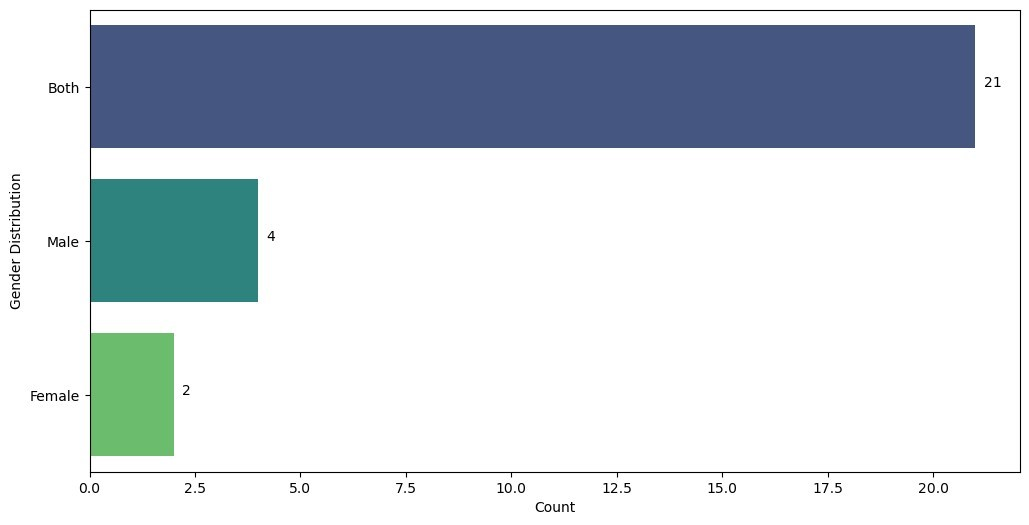
\includegraphics[width=\linewidth]{gender.jpg}
    \caption{Gender Distribution in Research Studies}
    \label{fig:prisma-flow-diagram6}
\end{figure}
However, 4 studies focused exclusively on male participants while only 2 studies examined female-only populations. The male-predominant pattern in single-gender studies may reflect occupational segregation in certain industries or historical biases in occupational health research. The limited number of studies conducted exclusively for women represents a missed opportunity to examine gender-specific factors such as hormonal influences, pregnancy-related metabolic changes, or challenges to work-life balance that can uniquely affect metabolic health in women.\par
The predominance of mixed-gender studies strengthens the generalizability of findings but may mask important gender-specific mechanisms or intervention responses that could inform targeted workplace health programs.

\subsection{Dietary Assessment Approaches and Nutritional Focus}
The analysis of dietary assessment patterns (Figure ~\ref{fig:prisma-flow-diagram7}) reveals significant limitations in nutritional evaluation within workplace metabolic syndrome research. The predominant category, "Unspecified Diet Patterns" (11 studies), indicates that many studies did not systematically assess dietary factors, representing a critical research gap given the fundamental role of nutrition in metabolic syndrome development.
\begin{figure}[H]
    \centering
    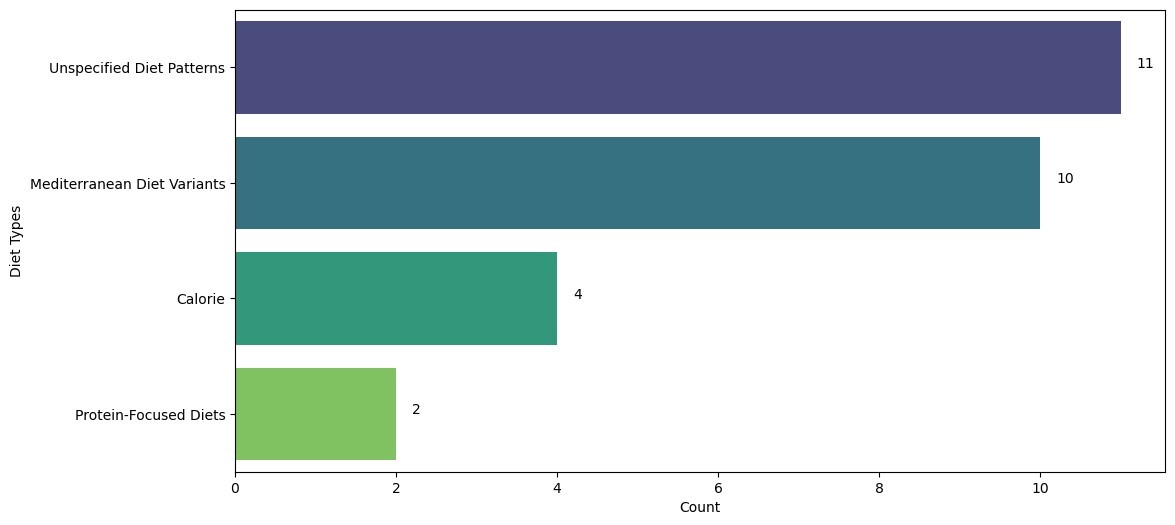
\includegraphics[width=\linewidth]{diet.jpg}
    \caption{Types of Dietary Assessments Used in Studies}
    \label{fig:prisma-flow-diagram7}
\end{figure}
Mediterranean Diet Variants were examined in 10 studies, reflecting growing recognition of this dietary pattern's protective effects against metabolic dysfunction. The emphasis on Mediterranean dietary approaches suggests research focus on evidence-based nutritional interventions with established cardiovascular and metabolic benefits.\par
Calorie-focused assessments appeared in 4 studies, while protein-focused dietary evaluations were conducted in only 2 studies. The limited attention to specific macro-nutrient patterns or alternative dietary approaches suggests that workplace nutrition research remains relatively narrow in scope.\par
The predominance of unspecified dietary assessments represents a significant methodological limitation, particularly given evidence that workplace environments can significantly influence eating behaviors through cafeteria options, time constraints, stress-related eating, and social influences on food choices.

\subsection{Age Demographics and Target Populations}
The age distribution analysis (Figure ~\ref{fig:prisma-flow-diagram8}) reveals a pronounced focus on middle-aged and older working adults, with individuals aged 45 and above comprising the largest study population (approximately 14 studies). This demographic emphasis is particularly significant given that metabolic syndrome prevalence increases with age and workplace responsibilities typically intensify in these age groups.

\begin{figure}[H]
    \centering
    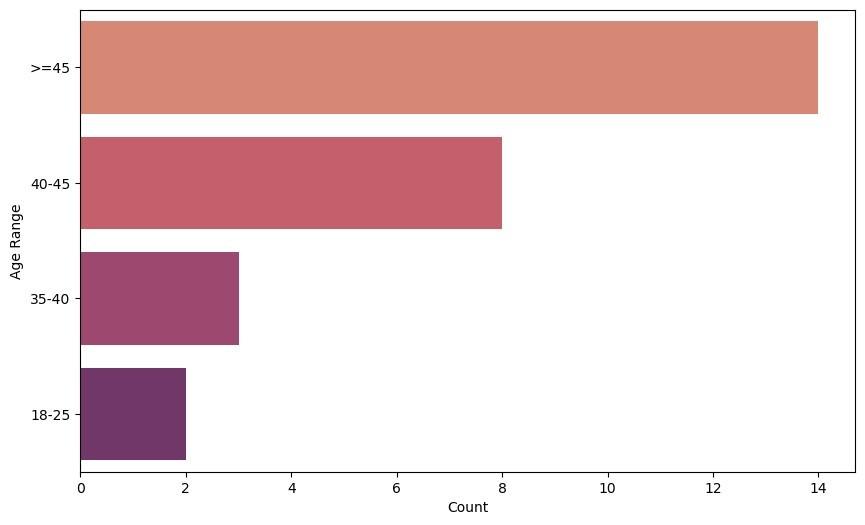
\includegraphics[width=\linewidth]{age.jpg}
    \caption{Age Range Distribution}
    \label{fig:prisma-flow-diagram8}
\end{figure}
The 40-45 age group represents the second-largest population (approximately 8 studies), followed by the 35-40 age range (approximately 3 studies). The minimal representation of younger workers (18-25 age group with approximately 2 studies) suggests a research gap in understanding early-career metabolic health patterns. This distribution pattern reflects the clinical reality that metabolic syndrome typically manifests in middle age, but may overlook important preventive opportunities in younger populations.

\subsection{Physical Activity Assessment Methodologies}
The methodological approaches for measuring physical activity (Figure ~\ref{fig:prisma-flow-diagram9}) demonstrate a strong preference for subjective assessment tools. Validated questionnaires and self-reports dominate the measurement landscape (approximately 10 studies), reflecting their practical feasibility in large-scale workplace research. Supervised exercise protocols represent the second most common approach (approximately 8 studies), suggesting efforts to maintain measurement consistency across studies.

\begin{figure}[H]
    \centering
    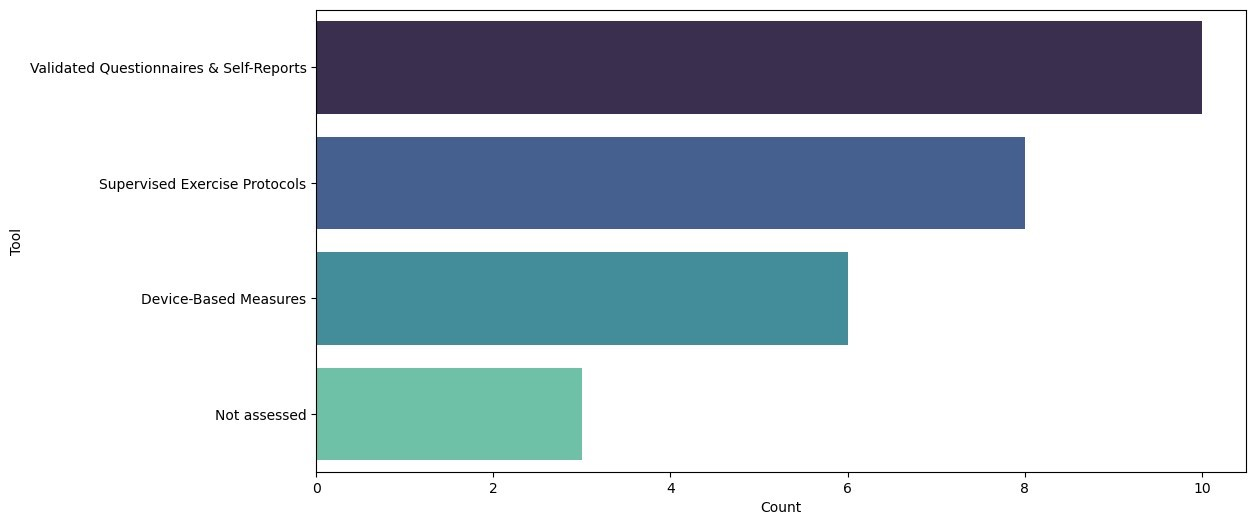
\includegraphics[width=\linewidth]{physical.jpg}
    \caption{Physical Activity Measurement Tools}
    \label{fig:prisma-flow-diagram9}
\end{figure}
Device-based measures, despite their objectivity, were employed in only about 6 studies, likely due to cost and logistical constraints in workplace settings. Notably, approximately 4 studies did not assess physical activity, representing a significant methodological limitation given the central role of physical activity in metabolic syndrome development. This measurement pattern highlights the ongoing challenge of balancing research feasibility with methodological rigor in workplace health studies.

\subsection{Measurement Tools and Research Focus}
The comprehensive analysis of measurement tools (Figure ~\ref{fig:measure}) reveals metabolic syndrome as the primary research focus, with approximately 13 studies directly measuring metabolic syndrome components. This central focus aligns with the review objectives and demonstrates the field's commitment to comprehensive metabolic health assessment.

\begin{figure}[H]
    \centering
    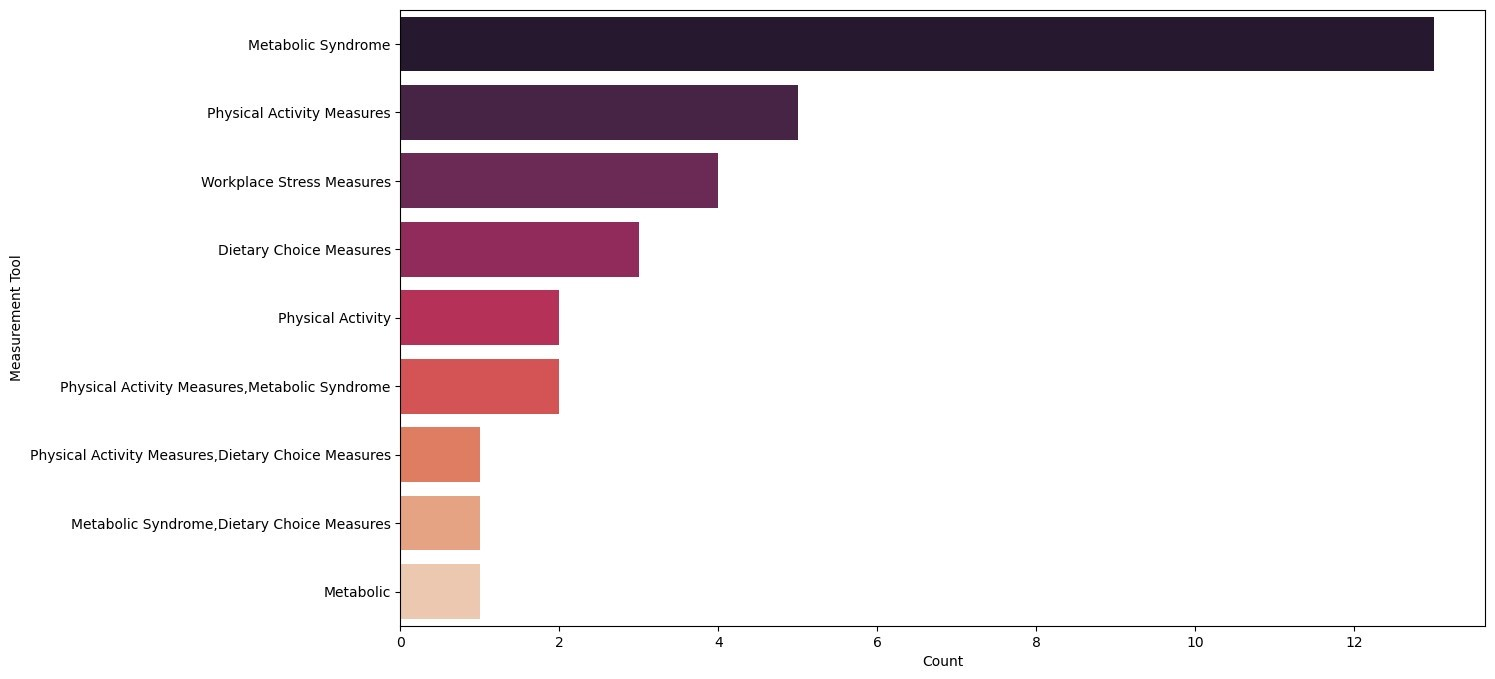
\includegraphics[width=\linewidth]{measure.jpg}
    \caption{Top 15 Measurement Tools Used }
    \label{fig:measure}
\end{figure}
Physical activity measures appear in approximately 6 studies, while workplace stress measures are employed in about 4 studies. Dietary choice measures are utilized in approximately 3 studies. Additional measurement combinations include studies examining both physical activity and metabolic syndrome (approximately 2 studies), and integrated approaches measuring physical activity and dietary choices (approximately 1 study).\par
This distribution pattern suggests potential research imbalances, with physical activity receiving more attention than workplace stress or dietary factors, despite the review's emphasis on their interconnected roles. The relatively lower frequency of workplace stress and dietary assessment tools indicates important research gaps. Given that chronic workplace stress can trigger both dietary changes and reduced physical activity, the under-representation of stress measurement tools may limit understanding of the complex pathways leading to metabolic syndrome in working populations.

\subsection{Study Design Characteristics and Methodological Quality}
The predominance of randomized controlled trials (RCTs) with 20 studies (Figure ~\ref{fig:design}) demonstrates the field's commitment to high-quality evidence generation. RCTs provide the strongest evidence for causal relationships between workplace interventions and metabolic outcomes, suggesting that researchers recognize the importance of rigorous methodology in this complex research area.
\begin{figure}[H]
    \centering
    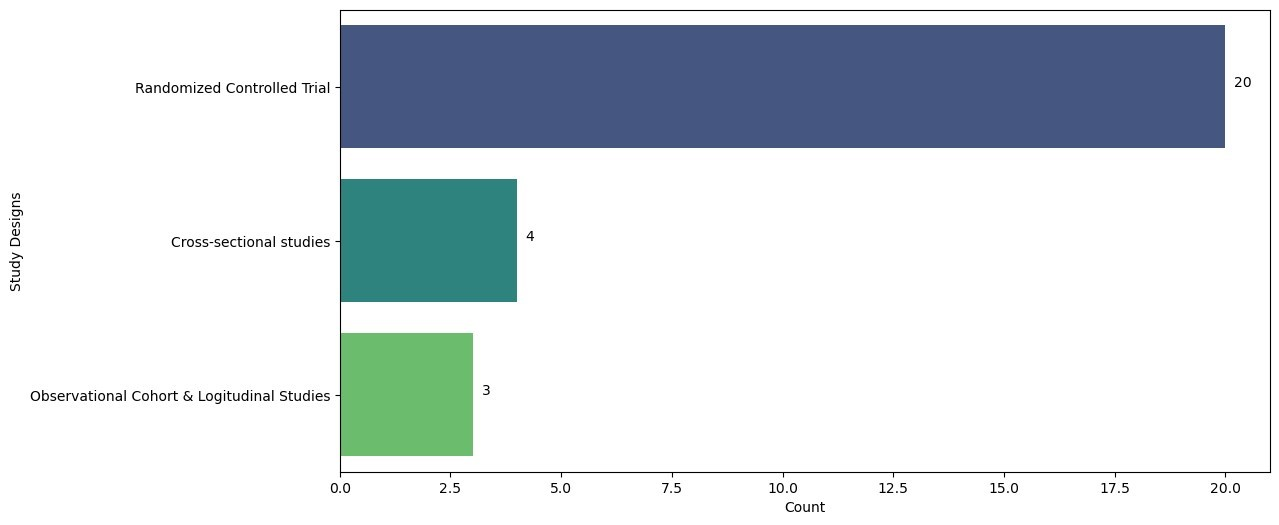
\includegraphics[width=\linewidth]{design.jpg}
    \caption{Top 10 Study Designs }
    \label{fig:design}
\end{figure}
Cross-sectional studies comprise 4 studies, offering valuable insights into population level associations but limiting causal inference capabilities. Observational cohort and longitudinal studies, with 3 studies, provide crucial temporal information about metabolic syndrome development over time, though their relative scarcity represents a notable limitation given the chronic nature of metabolic syndrome.
The heavy emphasis on experimental designs (RCTs) suggests that much research in this field focuses on intervention effectiveness rather than natural history or observational epidemiology. Although this approach supports evidence-based workplace health programs, it may limit understanding of how metabolic syndrome naturally develops in workplace contexts.

\section{Chi-Square Tests of Association Between Study Variables}
The following table summarizes the chi-square test results for ten selected pairs of categorical variables from the included studies, including degrees of freedom (df), p-values, Monte Carlo p-values where applicable, and interpretations.

\begin{table}[h!]
\centering
\caption{Chi-square test results for selected categorical variable pairs}
\label{tab:chi_square_results}

\begin{tabularx}{\textwidth}{|X|>{\centering\arraybackslash}m{1.2cm}|>{\centering\arraybackslash}m{1.2cm}|>{\centering\arraybackslash}m{1.5cm}|>{\centering\arraybackslash}m{2cm}|X|}
\hline
\textbf{Variable pair} & \textbf{$\chi^2$} & \textbf{df} & \textbf{p-value} & \textbf{Monte Carlo p} & \textbf{Conclusion} \\
\hline
Workplace $\times$ age range & 11.3237 & 12 & 0.5014 & 0.5446 & There is no significant association . \\
Workplace $\times$ gender & 22.9675 & 8 & 0.0034 & 0.0085 & There is significant association \\
Workplace $\times$ diet type & 18.6992 & 12 & 0.0961 & 0.0806 & There is no significant association \\
Age range $\times$ gender & 3.7825 & 6 & 0.7061 & 0.7269 & There is no significant association. \\
Age range $\times$ prevalent or incident rate & 74.6357 & 57 & 0.0585 & 0.0172 & There is  significant association \\
Gender $\times$ dietary assessment pattern & 9.6116 & 4 & 0.0475 & 0.0201 & There is significant association   \\
Diet type $\times$ prevalent or incident rate & 59.8827 & 57 & 0.3715 & 0.4536 & There is no significant association. \\
Duration $\times$ intensity level (physical activity) & 81.0000 & 78 & 0.3857 & 1.0000 & There is no significant association. \\
Measure tool used category $\times$ age range & 9.0643 & 6 & 0.1700 & 0.1658 & There is no significant association. \\
Prevalent or incident rate $\times$ measure tool used category & 37.2600 & 38 & 0.5035 & 0.6289 & There is no significant association. \\
\hline
\end{tabularx}
\end{table}
\newpage
To explore potential associations between categorical variables in the study, Pearson's chi-square tests were performed for selected variable pairs. This method was chosen because it is appropriate for testing relationships between two categorical variables without assuming a normal distribution. A significance level of 5\% ($\alpha$ = 0.05) was adopted; thus, p-values less than 0.05 were interpreted as evidence of a statistically significant association. In instances where more than 20\% of the expected cell counts were less than 5 and/or the minimum expected count was below 1, the assumptions of the Pearson chi-square test were violated. Under such conditions, the chi-square approximation becomes unreliable; therefore, the Monte Carlo simulation method was employed to obtain more accurate p-values.

Table~\ref{tab:chi_square_results} presents the chi-square test results for the selected variable pairs. The results indicated that workplace type and age range were not significantly associated (Monte Carlo p = 0.5446), suggesting that participant age distribution was similar across workplace settings. However, a significant association was observed between workplace type and gender (Monte Carlo p = 0.0085), indicating that gender composition varied across workplace categories. Workplace type and diet type had no significant association (Monte Carlo p = 0.0806), implying that dietary preferences did not differ by workplace setting.

Similarly, no significant association was found between age range and gender (Monte Carlo p = 0.7269), suggesting a balanced gender distribution across age groups. In contrast, age range and prevalent/incident status showed a significant association (Monte Carlo p = 0.0172), indicating that the occurrence of the condition varied with age group. The relationship between gender and dietary assessment pattern was statistically significant (Monte Carlo p = 0.0201).

The findings further revealed that diet type and prevalent/incident status were not significantly associated (Monte Carlo p = 0.4536), suggesting that dietary patterns were not linked with differences in prevalence or incidence rates. No significant relationships were found between physical activity duration and intensity level (Monte Carlo p = 1.0000), measurement tool category and age range (Monte Carlo p = 0.1658), or prevalent/incident status and measurement tool category (Monte Carlo p = 0.6289).

Overall, significant associations were identified for workplace and gender, age range and prevalent/incident status, and gender and dietary assessment patterns, while the remaining variable pairs showed no statistical evidence of association. These findings highlight the influence of workplace setting, age group, and dietary choices on study outcomes, while other factors such as physical activity patterns and measurement tools did not appear to vary meaningfully across the groups examined. 


\section{Synthesis of Key Findings}
\subsection{Workplace Stress and Metabolic Risk Factors}
The analysis reveals that workplace stress assessment tools are significantly underutilized relative to their theoretical importance in metabolic syndrome development. With 11 studies not assessing stress at all, this represents a critical methodological gap. Chronic occupational stress can trigger hormonal changes that promote abdominal obesity, insulin resistance, and dyslipidemia through cortisol-mediated pathways. The limited focus on stress measurement may reflect methodological challenges in quantifying workplace stress or insufficient recognition of its metabolic impact.\par
The geographic concentration of research in developed countries (USA and Italy leading with 5 and 4 studies respectively) may also influence understanding of stress-metabolism relationships, as workplace cultures and stressor profiles vary significantly across different economic and cultural contexts.
\subsection{Physical Activity Patterns and Interventions}
Physical activity emerges as the most frequently measured lifestyle factor, with validated questionnaires and self-reports predominating in 10 studies, followed by supervised exercise protocols in 8 studies. This reflects strong evidence for physical activity's protective effects against metabolic syndrome. However, the preference for self-report measures, while practical, may introduce measurement bias and limit precision in dose-response relationships. The substantial number of RCTs focusing on physical activity interventions suggests promising evidence for workplace-based exercise programs in metabolic syndrome prevention and management.\par
The diversity of workplace settings, particularly the inclusion of sports and tactical professions (3 studies), provides valuable insights into how different occupational physical demands may influence metabolic health outcomes differently than traditional sedentary work environments.
\subsection{Dietary Choices and Metabolic Outcomes}
Dietary assessment appears less frequently than expected given the fundamental role of nutrition in metabolic syndrome development, with 11 studies providing unspecified dietary assessments. However, the focus on Mediterranean Diet Variants in 10 studies demonstrates recognition of evidence-based nutritional approaches. This gap may reflect the complexity of dietary assessment in workplace settings or the challenge of implementing dietary interventions in occupational contexts. The limited attention to diverse dietary factors represents a significant research opportunity, particularly given the potential for workplace nutrition programs and the influence of workplace environments on eating behaviors.
\subsection{Age-Related Considerations}
The concentration of research on middle-aged and older workers aligns with metabolic syndrome epidemiology but may miss important preventive opportunities. The predominance of participants aged 45 and above (14 studies) versus minimal representation of younger workers aged 18-25 (2 studies) suggests that current research focuses more on treatment than prevention. Early-career interventions could potentially prevent metabolic syndrome development rather than merely managing established disease, particularly given the diverse workplace settings identified in the analysis.








